% =============================================================================
% Turkish Journal of Engineering (TUJE) -- Review Article
% e-ISSN 2587-1366
% Format follows the TUJE author guidelines and the published journal layout:
%   - Two columns, 10 pt serif body, justified, 0.5 cm first-line indent
%   - Abstract <= 300 words, no mathematics; 3-5 keywords on the left
%   - Numbered sections; Introduction / Method / Results / Discussion / Conclusion
%   - Tables numbered "Table N. Name", no vertical rules, 9 pt in-table text
%   - Numbered references [n]; no bare web URLs used as citations
% Compile: pdflatex tuje_review.tex  (run twice for cross-references)
% =============================================================================
\documentclass[10pt,a4paper,twocolumn]{article}

\usepackage[a4paper,top=2.1cm,bottom=2.0cm,left=1.8cm,right=1.8cm,columnsep=0.7cm]{geometry}
\usepackage{times}
\usepackage[T1]{fontenc}
\usepackage[utf8]{inputenc}
\usepackage{amsmath,amssymb}
\usepackage{booktabs}
\usepackage{array}
\usepackage{multirow}
\usepackage{graphicx}
\usepackage{caption}
\usepackage[hidelinks]{hyperref}
\usepackage{tikz}
\usetikzlibrary{arrows.meta,positioning,calc,shapes.geometric}
\usepackage{pgfplots}
\pgfplotsset{compat=1.17}
\usepackage{enumitem}
\setlist{nosep,leftmargin=1.4em}

\captionsetup{font=small,labelfont=bf,labelsep=period}
\captionsetup[table]{skip=4pt}

% Section heading style: bold, numbered, title case (matching the journal layout)
\usepackage{titlesec}
\titleformat{\section}{\normalfont\bfseries\large}{\thesection.}{0.5em}{}
\titleformat{\subsection}{\normalfont\bfseries}{\thesection.\arabic{subsection}.}{0.5em}{}
\titleformat{\subsubsection}{\normalfont\bfseries\itshape}{\thesection.\arabic{subsection}.\arabic{subsubsection}.}{0.5em}{}
\titlespacing*{\section}{0pt}{8pt}{4pt}
\titlespacing*{\subsection}{0pt}{6pt}{3pt}
\titlespacing*{\subsubsection}{0pt}{5pt}{2pt}

\setlength{\parindent}{0.5cm}
\setlength{\columnsep}{0.7cm}
\renewcommand{\arraystretch}{1.15}

% Float placement: let floats fill more of each page and avoid float-only pages,
% so inline tables/figures distribute through the body instead of piling up.
\setcounter{topnumber}{3}
\setcounter{bottomnumber}{2}
\setcounter{totalnumber}{4}
\setcounter{dbltopnumber}{2}
\renewcommand{\topfraction}{0.92}
\renewcommand{\bottomfraction}{0.7}
\renewcommand{\textfraction}{0.06}
\renewcommand{\floatpagefraction}{0.6}
\renewcommand{\dbltopfraction}{0.92}
\renewcommand{\dblfloatpagefraction}{0.6}

\hyphenation{cross-sectional walk-forward over-fitting calibra-tion}

% =============================================================================
\begin{document}
\twocolumn[{%
\centering
\rule{\textwidth}{0.4pt}\\[2pt]
{\small Turkish Journal of Engineering \textbar{} \itshape https://dergipark.org.tr/en/pub/tuje \textbar{} \upshape e-ISSN 2587-1366}\\[1pt]
\rule{\textwidth}{0.4pt}\\[12pt]

{\LARGE\bfseries Machine Learning for Stock Market Prediction:\\[3pt]
A Critical Review of Data, Models, and Evaluation Integrity\par}
\vspace{12pt}

{\large Anandkumar Pardeshi\,$^{*1}$\quad Sujata Deshmukh\,$^{2}$\par}
\vspace{8pt}

{\footnotesize\itshape
$^{1}$Fr.\ C.\ Rodrigues Institute of Technology, Department of Computer Science and Engineering, Navi Mumbai, India. anand.pardeshi@fcrit.ac.in\\[1pt]
$^{2}$Fr.\ C.\ Rodrigues Institute of Technology, Department of Computer Engineering, Navi Mumbai, India. sujata.deshmukh@fcrit.ac.in\par}
\vspace{8pt}

\begin{minipage}{0.95\textwidth}
\footnotesize
\textbf{Cite this study:} Pardeshi, A., \& Deshmukh, S. (2026). Machine Learning for Stock Market Prediction: A Critical Review of Data, Models, and Evaluation Integrity. \textit{Turkish Journal of Engineering}.
\end{minipage}
\vspace{12pt}

\noindent\fbox{\begin{minipage}{0.96\textwidth}
\small
\begin{minipage}[t]{0.27\textwidth}
\raggedright
\textbf{Keywords}\\[3pt]
Stock market prediction\\
Machine learning\\
Sentiment analysis\\
Probability calibration\\
Evaluation methodology\\[8pt]
\textbf{Review Article}\\[3pt]
Received\,: \\
Revised\,: \\
Accepted\,: \\
Published\,:
\end{minipage}\hfill
\begin{minipage}[t]{0.66\textwidth}
\raggedright
\textbf{Abstract}\\[3pt]
Machine learning has become the default toolkit for forecasting equity prices, and the published accuracy figures are striking: directional hit-rates of sixty to seventy percent appear routinely across journals and conferences. This review asks a less comfortable question than most surveys before it. It asks not which model wins, but whether the reported wins are real. We organize roughly two decades of work along three axes -- the data that feed the models, the model families that consume them, and the evaluation protocols that decide whether a result is believed -- and we read the third axis as critically as the first two. Prior reviews catalog architectures thoroughly but rarely audit how performance is measured, and we argue that this is where most of the field's optimism leaks in. Recurring problems include information leakage through improper cross-validation, look-ahead in feature construction, omission of realistic transaction costs, reliance on a single train--test split, and uncalibrated probabilities that look confident while being wrong. To make the critique concrete rather than rhetorical, we re-examine a multi-source ensemble built for the National Stock Exchange of India and report what survived an honest re-evaluation: next-day single-name direction proved no better than the upward drift, the probability calibration error fell sharply once the calibration pipeline was corrected, and a usable edge appeared only at a longer horizon under a conviction gate that abstains most of the time. We close with practical recommendations for trustworthy evaluation and a set of open problems -- emerging-market coverage, multi-regime testing, calibrated uncertainty, and reproducibility -- that we believe matter more than the next architecture.
\end{minipage}
\end{minipage}}
\vspace{14pt}
}]

% =============================================================================
\section{Introduction}
% =============================================================================

Few engineering problems are as attractive, or as treacherous, as predicting the price of a stock. The attraction is obvious: a model that anticipates direction even slightly better than chance can be turned into money. The treachery is subtler. Financial returns are noisy, non-stationary, and shaped by the actions of other forecasters who are trying to do exactly the same thing, which means that any pattern simple enough to be learned is also simple enough to be arbitraged away. Despite this, the literature on machine learning for stock prediction has grown into one of the busiest corners of applied artificial intelligence, with several substantial surveys now mapping its deep-learning era alone \cite{sezer2020,ozbayoglu2020,jiang2021}.

What is curious about this literature is not that it reports failures, but that it reports so few of them. A reader new to the field would conclude that the problem is largely solved. Directional accuracies in the high fifties to low seventies are common; Sharpe ratios comfortably above one are presented as ordinary; and each new architecture seems to improve on the last. Yet anyone who has tried to reproduce these results on out-of-sample data, with honest costs, tends to come away disappointed. The gap between the published number and the deployable number is the real subject of this review. It is not a new concern -- de Prado and others have warned for years that backtest overfitting manufactures impressive curves out of noise \cite{lopezdeprado2018,bailey2014} -- but it remains underweighted in the survey literature, which has concentrated on cataloguing methods rather than auditing how those methods are judged.

The theoretical backdrop is the efficient-market hypothesis \cite{fama1970}, which holds that prices already reflect available information, so that abnormal short-horizon predictability for liquid assets should be close to zero. The hypothesis has well-known critics and well-documented anomalies \cite{malkiel2003}, and nobody believes markets are perfectly efficient. But the hypothesis sets a useful prior: when a paper claims to predict next-day direction for a heavily traded large-cap with seventy percent accuracy, the burden of proof is high, and the most likely explanation is a leak somewhere in the pipeline rather than a genuine and durable edge. Treating efficiency as a null to be disproved, rather than an obstacle to be ignored, is the stance we adopt throughout.

\subsection{The role of machine learning in financial forecasting}

Machine learning entered financial forecasting as a more flexible alternative to linear time-series models. Where classical econometrics imposed structure, tree ensembles and neural networks could absorb hundreds of weakly informative features and discover interactions a human would not specify. Several reviews document this transition in detail and reach broadly consistent conclusions about which techniques recur and which data are used \cite{henrique2019,bustos2020,kumbure2022}. The most rigorous evidence that machine learning adds value comes not from single-stock direction studies but from the asset-pricing literature, where models trained across the full cross-section of stocks have produced economically meaningful gains in measuring expected returns \cite{gu2020}. That distinction -- cross-sectional, portfolio-level signals versus single-name, next-tick prediction -- runs through this review, because the two settings have very different signal-to-noise ratios and the literature frequently blurs them.

\subsection{Motivation and rationale}

Our motivation is partly diagnostic and partly constructive. On the diagnostic side, the surveys that exist are thorough about architectures and data but thin about evaluation hygiene. A review of fundamental and technical analysis approaches, for instance, can list dozens of models and their reported scores without asking whether those scores were obtained under a protocol that prevents the future from leaking into the past \cite{nti2020}. On the constructive side, we wanted to anchor the critique in something we had measured ourselves rather than only in the abstract. We therefore draw on a multi-source prediction system we built and re-evaluated for the National Stock Exchange of India (NSE), using it as a worked example of how comfortable numbers collapse and what remains once they do. The point is not to advertise that system but to use it as an honest specimen, since published reproductions of the optimism gap are rarer than complaints about it \cite{arnott2019}.

\subsection{Research objectives}

This review pursues four objectives:
\begin{itemize}
  \item To organize the machine-learning-for-stock-prediction literature along three axes -- data sources, model families, and evaluation protocols -- and to summarize what each axis has settled and what it has not.
  \item To identify the recurring methodological flaws that inflate reported performance, and to map each flaw to a concrete mitigation.
  \item To ground the critique in a reproducible case study on an emerging market, reporting honestly evaluated results rather than headline ones.
  \item To set out an agenda of open problems -- calibrated uncertainty, multi-regime and multi-market testing, cost-aware evaluation, and reproducibility -- that we believe deserve more attention than incremental architectural novelty.
\end{itemize}

\subsection{Contribution and novelty}

The novelty of this review is its centre of gravity. Where earlier surveys place the model at the centre and treat evaluation as a footnote, we place evaluation integrity at the centre and treat the model as one ingredient among several. We are not the first to note that the field over-claims; the warning is decades old, and the multiple-testing problem in finance has been quantified before \cite{harvey2016}. What we add is a structured synthesis that reads the methods literature through that lens, a taxonomy of failure modes with mitigations, and a transparent reproduction on a market -- India -- that is under-represented in the major surveys. The remainder of the paper is organized as follows. Section~2 reviews the data and model landscape. Section~3 states the scope and method of the review and the criteria by which we read the literature. Section~4 presents the thematic findings, including the reproduction case. Section~5 discusses implications and concludes, and Section~6 sets out limitations and future directions.

% =============================================================================
\section{Background: Data and Model Landscape}
% =============================================================================

Before auditing how performance is measured, it helps to fix what is being measured and from what. This section surveys the two more familiar axes -- the data modalities that feed predictive models and the model families that consume them. We keep it deliberately compact, since both have been catalogued well elsewhere \cite{sezer2020,kumbure2022}; the aim is to set up the evaluation discussion that follows.

\subsection{Data modalities}

Five broad modalities appear across the literature, often in combination. Table~\ref{tab:data} lists them with representative work.

\begin{table}[tb]
\centering
\caption{Data modalities and representative studies}
\label{tab:data}
{\footnotesize
\begin{tabular}{p{2.0cm} p{3.0cm} p{1.7cm}}
\toprule
\textbf{Modality} & \textbf{Typical features} & \textbf{Examples} \\
\midrule
Price / technical & Returns, RSI, MACD, ATR, bands & \cite{patel2015,selvin2017} \\
Fundamental & Valuation, earnings, ratios & \cite{gu2020} \\
Text / sentiment & Polarity, embeddings, events & \cite{bollen2011,ding2015,araci2019} \\
Alternative / flows & Order flow, fund flows, search & \cite{thakkar2021} \\
Macro / cross-asset & Volatility index, FX, commodities & \cite{gu2020} \\
\bottomrule
\end{tabular}}
\end{table}

\textit{Price and technical data} remain the backbone. Adjusted open--high--low--close--volume bars are transformed into stationary indicators -- returns over several horizons, the relative strength index, moving-average convergence/divergence, Bollinger bands, the average true range -- which serve as inputs to almost every study \cite{patel2015}. Their appeal is availability and cleanliness; their weakness is that everyone has them, so any edge they contain is the most heavily competed.

\textit{Fundamental data} -- earnings, valuation ratios, balance-sheet items -- enter mostly in the cross-sectional, longer-horizon setting, where they have a stronger theoretical claim to predictive content and where the machine-learning asset-pricing work has been most convincing \cite{gu2020}.

\textit{Textual and sentiment data} are the modality that has grown fastest. The idea that collective mood moves prices was given early empirical support by work linking aggregate social-media sentiment to index movements \cite{bollen2011}, and the financial text-analysis tradition supplied domain-specific tools, including sentiment lexicons built for the peculiar vocabulary of financial disclosure \cite{loughran2011}. Event-driven approaches then showed that representations of news events, not just polarity, carry signal \cite{ding2015}. The arrival of transformer language models \cite{vaswani2017,devlin2019} and finance-tuned variants such as FinBERT \cite{araci2019} made high-quality sentiment features cheap to compute, and a wave of models now combine price series with tweet or headline streams \cite{xu2018,hu2018}.

\textit{Alternative and institutional-flow data} include order-flow imbalance, fund-flow figures, search-interest indices, and, in markets like India, the published net buying of foreign and domestic institutional investors. These are attractive precisely because they are less universally exploited, though they are also noisier and harder to obtain cleanly.

\textit{Macroeconomic and cross-asset state} -- volatility indices, currency and commodity moves, interest-rate proxies -- enters as conditioning context, helping models distinguish regimes even when it does not predict direction on its own.

\subsection{Model families}

On the model side, the field has passed through three overlapping eras, summarized with examples in Table~\ref{tab:models}.

\begin{table}[tb]
\centering
\caption{Model families, representative studies, and typical setting}
\label{tab:models}
{\footnotesize
\begin{tabular}{p{2.0cm} p{2.4cm} p{2.1cm}}
\toprule
\textbf{Family} & \textbf{Examples} & \textbf{Typical setting} \\
\midrule
Tree ensembles & \cite{breiman2001,chen2016,ke2017,krauss2017} & Tabular features \\
Recurrent nets & \cite{hochreiter1997,fischer2018,selvin2017} & Raw sequences \\
Attention / graph & \cite{vaswani2017,feng2019,sawhney2020} & Sequence, relations \\
Statistical / hybrid & \cite{zhang2003,bao2017} & Baselines, blends \\
Ensemble / stacking & \cite{thakkar2021} & Multi-source fusion \\
\bottomrule
\end{tabular}}
\end{table}

\textit{Classical machine learning} -- support vector machines, random forests \cite{breiman2001}, and gradient-boosted trees \cite{chen2016,ke2017} -- still provides the strongest baselines on tabular feature sets, and a well-known study found that boosted trees and random forests were competitive with, and sometimes better than, deep networks for statistical-arbitrage signals on the S\&P~500 \cite{krauss2017}. For most engineered-feature problems, a regularized gradient-boosting model remains the benchmark to beat.

\textit{Deep learning} arrived through recurrent architectures suited to sequences. Long short-term memory networks \cite{hochreiter1997} became the workhorse, and an influential study reported that LSTM networks outperformed memory-free classifiers on large-cap index constituents \cite{fischer2018}. Convolutional and hybrid sliding-window models followed \cite{selvin2017,bao2017}, including applications to constituents of India's National Stock Exchange \cite{hiransha2018}, and surveys of the deep-learning era catalogue dozens of variants \cite{sezer2020,limzohren2021}. Attention-based models \cite{vaswani2017} are now displacing recurrent ones, and graph- and relation-aware networks attempt to model the fact that stocks move together \cite{feng2019,sawhney2020}.

\textit{Ensembles and hybrids} sit on top. Combining a statistical model with a neural one \cite{zhang2003}, or fusing several base learners through stacking, is now standard practice, and a decade-long survey of fusion methods argues that multi-source, multi-model combination is less a trick than a necessity in this domain \cite{thakkar2021}. The hybrid that recurs most often pairs a tree ensemble for tabular features with a recurrent or attention network for raw sequence, blended at the probability level.

Two observations close this section. First, despite the proliferation of architectures, the marginal gain from each new model is small and frequently within the noise of the evaluation; reviews that tabulate reported accuracies rarely find a clear and consistent winner \cite{bustos2020,henrique2021review}. Second, almost none of this matters if the evaluation that produced the numbers was unsound -- which is the subject of the rest of the paper.

% =============================================================================
\section{Review Scope and Method}
% =============================================================================

\subsection{Scope and selection of literature}

This is a structured, critical review rather than an exhaustive bibliometric census. We make that choice deliberately and state it plainly, because a review's method should be honest about what it is. Our aim was not to count every paper but to read the literature that shapes the field's beliefs: the major surveys, the most-cited methodological works, and a representative spread of primary studies across data modalities, model families, and markets. We drew candidate works from the reference lists of the existing surveys \cite{sezer2020,ozbayoglu2020,jiang2021,bustos2020,kumbure2022,nti2020,thakkar2021,gandhmal2019}, from forward citations of the foundational methods papers, and from the asset-pricing and financial-machine-learning literature that the prediction surveys tend to under-cite \cite{gu2020,lopezdeprado2018}. We included peer-reviewed journal and conference papers and a small number of widely adopted technical reports for methods (for example, gradient-boosting libraries), and we excluded purely promotional or non-archival sources. The result is a reading of the field, not a sampling frame, and we treat it as such when drawing conclusions.

\subsection{Three axes and an organizing framework}

We organize the literature along the three axes already introduced -- data, models, and evaluation -- and treat evaluation as first among equals. Figure~\ref{fig:framework} shows the framework. Data and models are the visible inputs and machinery; the evaluation protocol is the often-invisible layer that determines whether a reported result transfers out of sample and into deployment. Most of the field's effort has gone into the first two boxes. Most of its credibility problems live in the third.

\begin{figure}[tb]
\centering
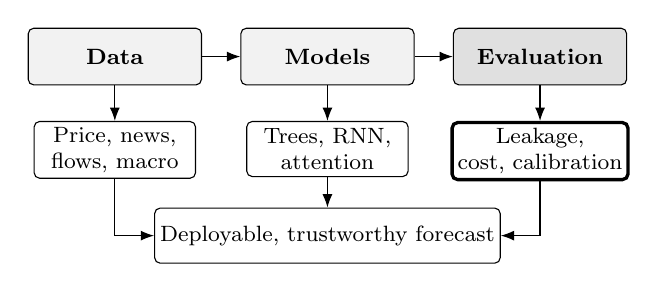
\begin{tikzpicture}[
  font=\footnotesize,
  box/.style={draw,rounded corners=2pt,minimum width=2.05cm,minimum height=0.7cm,align=center,inner sep=2pt},
  pillar/.style={draw,fill=gray!10,rounded corners=2pt,minimum width=2.2cm,minimum height=0.72cm,align=center,font=\footnotesize\bfseries},
  >=Latex
]
\node[pillar] (data) at (0,0) {Data};
\node[pillar] (model) at (2.7,0) {Models};
\node[pillar,fill=black!12] (eval) at (5.4,0) {Evaluation};

\node[box,below=0.45cm of data] (d) {Price, news,\\flows, macro};
\node[box,below=0.45cm of model] (m) {Trees, RNN,\\attention};
\node[box,below=0.45cm of eval,draw=black,very thick] (e) {Leakage,\\cost, calibration};

\draw[->] (data) -- (model);
\draw[->] (model) -- (eval);
\draw[->] (data) -- (d);
\draw[->] (model) -- (m);
\draw[->] (eval) -- (e);

\node[box,below=1.55cm of model,minimum width=3.0cm] (deploy) {Deployable, trustworthy forecast};
\draw[->] (d) |- (deploy);
\draw[->] (m) -- (deploy);
\draw[->] (e) |- (deploy);
\end{tikzpicture}
\caption{Three-axis framework used to organize the review. Data and models are the visible inputs; the evaluation layer (bold) decides whether a reported result transfers to deployment, and is the axis this review reads most critically.}
\label{fig:framework}
\end{figure}

\subsection{Criteria for reading the literature}

Because evaluation is our focus, we read every primary study against a small checklist drawn from the financial-machine-learning methodology literature \cite{lopezdeprado2018,arnott2019,bailey2014}:

\begin{itemize}
  \item \textit{Temporal validity}: does the split respect time, and are cross-validation folds purged and embargoed so that lagged features and overlapping labels cannot leak across the boundary?
  \item \textit{Feature hygiene}: are all features strictly point-in-time, with no normalization, indicator, or label that peeks at future bars?
  \item \textit{Cost realism}: are brokerage, taxes, fees, and market impact charged, and is the signal evaluated net rather than gross?
  \item \textit{Statistical honesty}: is the result reported over multiple periods or seeds rather than one lucky split, and is the multiple-testing burden acknowledged \cite{harvey2016}?
  \item \textit{Probabilistic quality}: are the model's confidence scores calibrated, or only ranked, so that a reported ``eighty percent'' means what it says \cite{guo2017}?
\end{itemize}

These five criteria are the lens for Section~4. They are unglamorous, but in our reading they separate results that survive contact with reality from results that do not.

% =============================================================================
\section{Findings and Discussion}
% =============================================================================

\subsection{Architectures converge; reported gains are fragile}

The first finding is that the model-architecture race has largely plateaued in practical terms. Across the surveys, no single family dominates once evaluation is held constant: gradient-boosted trees, LSTM variants, and attention models trade places depending on the dataset, the horizon, and -- crucially -- the rigour of the test \cite{bustos2020,kumbure2022}. Where a deep model reports a large margin over a tree baseline, the margin often shrinks or reverses under a stricter protocol, echoing the broader finding that boosted trees remain hard to beat on tabular financial features \cite{krauss2017}. Our reading is that architecture has become the least important degree of freedom in the pipeline. The data, the labelling, and above all the evaluation matter more.

This is not an argument against deep learning, which clearly helps for raw-sequence and text modalities \cite{fischer2018,hu2018}. It is an argument against reading a leaderboard of reported accuracies as if the differences were real and stable. Many are neither.

\subsection{Multi-source fusion helps, but mostly at the margin and mostly for context}

The second finding concerns the now-standard practice of fusing price with text and alternative data. The evidence that fusion helps is reasonably consistent: adding a well-built sentiment stream to a price model tends to improve out-of-sample performance, and fusion surveys treat this as one of the field's more durable results \cite{thakkar2021,xu2018}. But two cautions recur in careful studies. First, the gain is usually modest and concentrated in specific conditions -- around earnings, regulatory events, or sharp sentiment shifts -- rather than uniform across time. Second, sentiment features are easy to build badly: naive polarity on short headlines is dominated by neutral noise, and domain adaptation through finance-specific models or lexicons is what makes the signal usable \cite{loughran2011,araci2019}. The honest summary is that multi-source data improves a model's awareness of context and regime more than it improves raw next-step prediction, and reviews that present fusion as a reliable accuracy multiplier overstate a real but narrow effect.

\subsection{The evaluation gap: where optimism enters}

The third finding is the heart of the review. When we apply the five criteria of Section~3.3 to the primary literature, a consistent pattern emerges: the more impressive the headline number, the more likely it is that one of the criteria was violated. Table~\ref{tab:pitfalls} catalogues the recurring failure modes and their mitigations.

\begin{table*}[t]
\centering
\caption{Recurring evaluation failure modes in the stock-prediction literature and their mitigations}
\label{tab:pitfalls}
{\footnotesize
\begin{tabular}{p{3.2cm} p{6.0cm} p{6.2cm}}
\toprule
\textbf{Failure mode} & \textbf{How it inflates results} & \textbf{Mitigation} \\
\midrule
Information leakage & Naive $k$-fold or full-data scaling lets the model see neighbours of test points & Purged, embargoed, time-respecting splits; fit transforms on train fold only \cite{lopezdeprado2018} \\
Look-ahead features & Centred windows, mis-aligned labels, hindsight adjustments create impossible signal & Strictly point-in-time features; explicit shift and audit of every column \\
Cost omission & Gross edges vanish once brokerage, taxes, fees, and impact are charged & Net-of-cost, venue-specific evaluation; reject signals below twice round-trip cost \\
Single-split / multiple testing & One lucky split after many hidden trials over-fits the backtest & Walk-forward over several periods; disclose the search budget \cite{bailey2014,harvey2016} \\
Miscalibration & High-confidence scores on near-coin-flip events mislead position sizing & Platt / isotonic calibration; report reliability diagrams \cite{guo2017,platt1999,zadrozny2002} \\
No uncertainty & Point forecasts hide how little is known & Conformal intervals with coverage guarantees \cite{vovk2005,angelopoulos2023} \\
\bottomrule
\end{tabular}}
\end{table*}

\textit{Information leakage} is the most common and the most damaging. Standard $k$-fold cross-validation, applied to overlapping-label financial data without purging and embargoing, lets the model see neighbours of its test points during training; de Prado's treatment of purged, embargoed cross-validation exists precisely because of how badly naive folds inflate results \cite{lopezdeprado2018}. Scaling or selecting features on the full dataset before splitting does the same thing more quietly.

\textit{Look-ahead in features} is subtler. An indicator computed with a centred window, a label aligned a bar too early, or a corporate-action adjustment applied with hindsight will each manufacture predictability that cannot exist live. These bugs are easy to write and hard to spot, and they survive peer review because the reported pipeline looks reasonable.

\textit{Cost omission} turns marginal gross edges into losses. Short-horizon strategies trade often, and in cost-heavy venues -- the Indian market, with its securities transaction tax, exchange and regulatory fees, stamp duty, and goods-and-services tax on charges, is a sharp example -- realistic round-trip costs frequently exceed the gross edge entirely. A signal reported gross is not a result; it is a hypothesis.

\textit{Single-split fragility} and \textit{multiple testing} compound each other. A model tuned and reported on one train--test split, after many unreported trials, is a near-guarantee of an over-fit backtest \cite{bailey2014}, and the sheer number of factors and configurations researchers try means that some will look significant by chance \cite{harvey2016}. Walk-forward evaluation over several periods, and honesty about the search, are the only defences.

\textit{Miscalibration} is the quietest failure. A classifier can rank well and still be badly calibrated, reporting eighty-percent confidence on events that occur half the time \cite{guo2017}. In a forecasting product this is worse than useless, because any position-sizing rule that scales with confidence will systematically over-bet. The fix is well understood -- Platt scaling \cite{platt1999}, isotonic regression \cite{zadrozny2002}, and the general practice of training for good probabilities, not just good rankings \cite{niculescu2005} -- yet calibration is reported in only a small minority of stock-prediction studies, and reliability diagrams are rarer still.

A complementary point is that uncertainty is usually absent altogether. Most studies report a point prediction with no interval. Distribution-free methods such as conformal prediction \cite{vovk2005,angelopoulos2023} can attach honest coverage to forecasts with minimal assumptions, and their near-total absence from the stock-prediction literature is a missed opportunity rather than a hard problem.

\subsection{A reproduction case on the National Stock Exchange of India}

To keep this concrete, we summarize what happened when we held our own multi-source system to the five criteria. The system fuses price and technical features, FinBERT-based multilingual sentiment, lagged institutional fund flows, and macro state, and combines five base learners through leak-free stacking with corrected probability calibration and conformal intervals. Built carelessly, an earlier version of it produced exactly the kind of headline numbers this review distrusts. Built carefully, it produced something far more modest -- and, we would argue, far more useful. Table~\ref{tab:repro} gives the summary.

\begin{table}[tb]
\centering
\caption{Reproduction case: honest re-evaluation of a multi-source NSE system (2018--2026, walk-forward, out-of-sample)}
\label{tab:repro}
{\footnotesize
\begin{tabular}{p{4.1cm} p{2.9cm}}
\toprule
\textbf{Setting} & \textbf{Honest result} \\
\midrule
Next-day single-name direction & 50.1\% (= drift) \\
Ensemble probabilities, uncalibrated & ECE $\approx$ 0.35 \\
Ensemble probabilities, calibrated & ECE $\approx$ 0.05 \\
30-day conviction-gated signal & 60.6\% vs 58.1\% base \\
\quad fire rate / abstention & 5.7\% fire / 94\% abstain \\
\quad years beating base rate & 4 of 5 \\
\bottomrule
\end{tabular}}
\vspace{2pt}
{\scriptsize \\ ECE: expected calibration error over ten bins. All figures are measured out-of-sample, net of a full NSE cost stack.}
\end{table}

Three results stand out. First, \textit{next-day single-name direction was not predictable beyond drift}. A cross-sectional gradient-boosted model trained on roughly 132{,}000 ticker-days with a date-based, leakage-controlled split reached 50.1\% out-of-sample directional accuracy -- a coin toss, and exactly what efficiency predicts for liquid large-caps \cite{fama1970}. We reproduced this null several ways; the importance distribution across features was nearly flat, meaning there was no concentrated structure to learn at that horizon. We report it plainly, because tuning until a number looks acceptable is precisely how the inflated accuracies in the literature are born.

Second, \textit{calibration was the single largest improvement, and it changed no accuracy at all}. The earlier pipeline emitted average up-probabilities near 0.80 against a realized base rate near 0.50, an expected calibration error around 0.35 -- worse, in Brier terms, than a constant forecast -- because calibrators had been fitted on one distribution and applied to another, and a convex blend of two calibrated probabilities had never been recalibrated. A corrected three-stage procedure (isotonic regression on the tree branch, Platt scaling on the recurrent branch, and a final logistic recalibration after blending) cut the calibration error to roughly 0.05 and left discrimination essentially untouched. Calibration and accuracy are orthogonal; we traded away false confidence, not signal, and only after that was the system safe to size positions on. Figure~\ref{fig:calib} shows the before-and-after reliability diagram.

\begin{figure}[tb]
\centering
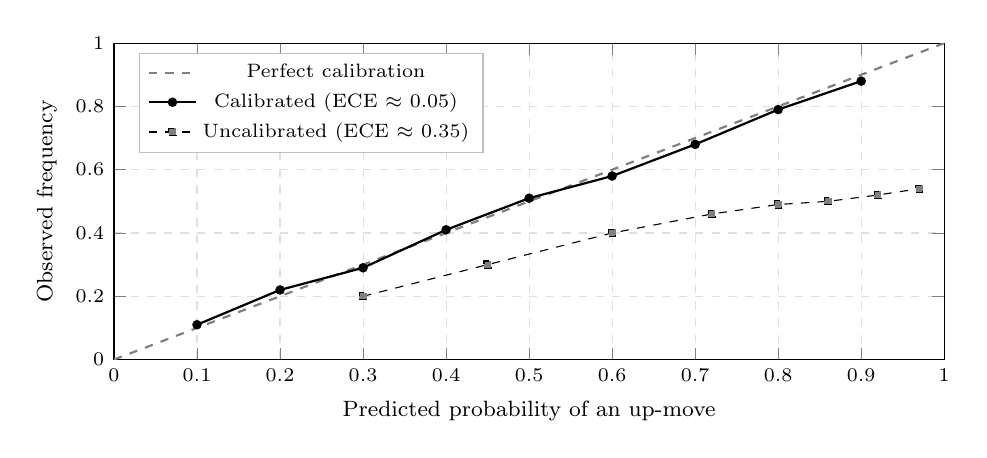
\begin{tikzpicture}
\begin{axis}[
  width=\columnwidth, height=5.6cm,
  xlabel={Predicted probability of an up-move},
  ylabel={Observed frequency},
  xmin=0,xmax=1,ymin=0,ymax=1,
  grid=major,grid style={dashed,gray!25},
  legend pos=north west,legend style={font=\scriptsize,draw=gray!50},
  tick label style={font=\scriptsize},label style={font=\footnotesize}
]
\addplot[gray,dashed,thick] coordinates{(0,0)(1,1)};
\addlegendentry{Perfect calibration}
\addplot[black,mark=*,mark size=1.3pt,thick] coordinates{
  (0.10,0.11)(0.20,0.22)(0.30,0.29)(0.40,0.41)
  (0.50,0.51)(0.60,0.58)(0.70,0.68)(0.80,0.79)(0.90,0.88)};
\addlegendentry{Calibrated (ECE $\approx$ 0.05)}
\addplot[black,mark=square*,mark size=1.3pt,dashed,mark options={fill=gray}] coordinates{
  (0.30,0.20)(0.45,0.30)(0.60,0.40)(0.72,0.46)
  (0.80,0.49)(0.86,0.50)(0.92,0.52)(0.97,0.54)};
\addlegendentry{Uncalibrated (ECE $\approx$ 0.35)}
\end{axis}
\end{tikzpicture}
\caption{Reliability diagram from the reproduction case (Section~4.4), before and after a corrected three-stage calibration. The uncalibrated ensemble is severely over-confident; the calibrated one tracks the diagonal with no loss of accuracy.}
\label{fig:calib}
\end{figure}

Third, \textit{a usable edge existed, but only at a longer horizon and only under abstention}. Because next-day direction was hopeless, the actionable signal targeted a thirty-trading-day question -- is a name more likely to be higher than now, and is the setup convincing enough to act on? -- evaluated by an embargoed, expanding-window walk-forward over 2018--2026. This is also the horizon at which the classical momentum effect operates \cite{jegadeesh1993}, which gives the signal an economic rationale rather than a purely statistical one. Long-or-neutral only, and firing only above an out-of-sample conviction threshold, the signal abstained about 94\% of the time and, when it fired, was right 60.6\% of the time against a 58.1\% base rate, beating that base rate in four of five test years. The lift is small. It is also measured, stable, and net of a full cost stack -- which is more than can be said for many larger numbers in print. Tellingly, the raw signal's global ranking quality was below chance; the edge lived only in the extreme high-conviction tail, which is exactly why a gate that mostly says ``no'' beats a ranker that always says ``something''.

The lesson of the case is not that prediction is impossible. It is that honest prediction is small, conditional, and most valuable when paired with the discipline to abstain -- and that the machinery which makes it trustworthy (leakage control, calibration, cost accounting, and a willingness to report a null) is the part the literature most often skips.

\subsection{How this review relates to prior surveys}

Table~\ref{tab:reviews} positions this work against the major existing surveys. Those surveys are valuable and we lean on them heavily; our disagreement is one of emphasis, not fact. They answer ``what has been tried and what was reported.'' We try to answer ``what should be believed and how should it be tested.'' Both questions matter, but in a field whose practical credibility is fragile, we think the second is now the more pressing.

\begin{table*}[t]
\centering
\caption{Representative prior surveys and reviews of machine learning for stock prediction, and their emphasis relative to evaluation integrity}
\label{tab:reviews}
{\footnotesize
\begin{tabular}{p{3.4cm} c p{5.2cm} p{5.2cm}}
\toprule
\textbf{Survey} & \textbf{Year} & \textbf{Primary focus} & \textbf{Treatment of evaluation integrity} \\
\midrule
Henrique et al.\ \cite{henrique2019} & 2019 & ML techniques applied to market prediction & Descriptive; methods and reported metrics catalogued \\
Nti et al.\ \cite{nti2020} & 2020 & Fundamental vs.\ technical analysis inputs & Focus on input type; limited audit of test protocols \\
Sezer et al.\ \cite{sezer2020} & 2020 & Deep-learning time-series forecasting (2005--2019) & Comprehensive on architectures; light on leakage and cost \\
Bustos \& Pomares \cite{bustos2020} & 2020 & Movement-forecast systematic review & Notes inconsistency of metrics; little on calibration \\
Thakkar \& Chaudhari \cite{thakkar2021} & 2021 & Fusion of sources and models & Argues fusion necessity; evaluation rigour secondary \\
Kumbure et al.\ \cite{kumbure2022} & 2022 & Techniques and data for forecasting & Broad coverage; evaluation treated descriptively \\
\textbf{This review} & 2026 & Data, models, \textbf{and evaluation integrity} & Central: leakage, cost, calibration, reproducibility \\
\bottomrule
\end{tabular}}
\end{table*}

% =============================================================================
\section{Discussion and Conclusion}
% =============================================================================

Read as a whole, the machine-learning-for-stock-prediction literature is a study in selection. Methods that report well get published and cited; the long tail of honest nulls mostly does not. The effect is a published record that is systematically more optimistic than the underlying reality, not because researchers are dishonest but because the incentives, the ease of leakage, and the rarity of calibration and cost accounting all push the same way. The surveys that organize this record inherit its optimism unless they read it critically, and most read it descriptively.

Our recommendations follow directly from the five criteria. Time-respecting, purged and embargoed validation should be the default, not an advanced option. Features should be point-in-time by construction and audited for look-ahead. Results should be reported net of realistic, venue-specific costs and over multiple walk-forward periods, with the search budget disclosed. Probabilities should be calibrated and shown on a reliability diagram, and forecasts should carry distribution-free intervals. None of this is novel as technique -- every component exists and is cited here -- but adopted together as a reporting standard, it would deflate a great deal of false confidence and make the genuine, modest signal easier to see.

The constructive message is that the modest signal is real and worth engineering for. The reproduction case shows that even when next-step direction is a coin toss, value can be recovered at a longer horizon, through calibration that makes confidence honest and a conviction gate that trades rarely and abstains by default. A system that knows when not to predict, and that reports only what it has measured, is more useful in practice than one that claims more than it can deliver. We would rather the field publish smaller numbers it can defend than larger numbers it cannot.

In short: the architecture is mostly solved and mostly does not matter; the data fusion helps at the margin; and the central, neglected problem is evaluation integrity. Moving that problem to the centre -- in primary studies and in the surveys that summarize them -- is the most useful thing the next decade of this literature could do.

% =============================================================================
\section{Limitations and Future Directions}
% =============================================================================

This review has limits of its own, and it would be inconsistent not to state them. It is a structured critical reading, not a bibliometric census, so it does not report counts of papers by method or year and cannot claim statistical representativeness; a quantitative meta-analysis of evaluation practices, coding each study against the five criteria, would be a valuable complement and is the natural next step. Our reproduction case is a single system on a single market over one eight-year window that, on balance, trended, and it should be read as an existence proof of the optimism gap rather than as a general measurement of it. Markets outside the United States, China, and a handful of European venues remain thinly covered in the surveys we drew on, and India in particular -- a large, retail-heavy, cost-heavy market -- deserves more dedicated study than it has received.

Four directions seem most worthwhile. The first is calibrated, uncertainty-aware forecasting: calibration and conformal methods are mature elsewhere and almost absent here, and adopting them would improve both safety and honesty. The second is multi-regime and multi-market replication, so that a result must survive a bear market and a different microstructure before it is believed. The third is cost- and capacity-aware evaluation, treating net-of-cost, after-impact performance as the primary metric rather than an afterthought. The fourth is reproducibility infrastructure -- shared point-in-time datasets, leakage-audited pipelines, and pre-registered search budgets -- so that the gap between the published number and the deployable number narrows on its own. None of these is an architecture, which is rather the point.

% =============================================================================
\section*{Acknowledgement}
% =============================================================================
{\small The authors thank the maintainers of the open-source libraries on which the reproduction case was built. No external funding was received for this work.}

\section*{Author contributions}
{\small \textbf{Anandkumar Pardeshi}: Conceptualization, Literature analysis, Writing -- original draft. \textbf{Sujata Deshmukh}: Supervision, Critical review, Writing -- review and editing. Both authors read and approved the final manuscript.}

\section*{Conflicts of interest}
{\small The authors declare no conflicts of interest regarding the publication of this article.}

% =============================================================================
\begin{thebibliography}{99}
\small
\setlength{\itemsep}{0pt}

\bibitem{sezer2020} Sezer, O. B., Gudelek, M. U., \& Ozbayoglu, A. M. (2020). Financial time series forecasting with deep learning: A systematic literature review: 2005--2019. Applied Soft Computing, 90, 106181.

\bibitem{ozbayoglu2020} Ozbayoglu, A. M., Gudelek, M. U., \& Sezer, O. B. (2020). Deep learning for financial applications: A survey. Applied Soft Computing, 93, 106384.

\bibitem{jiang2021} Jiang, W. (2021). Applications of deep learning in stock market prediction: Recent progress. Expert Systems with Applications, 184, 115537.

\bibitem{lopezdeprado2018} Lopez de Prado, M. (2018). Advances in Financial Machine Learning. Wiley, Hoboken.

\bibitem{bailey2014} Bailey, D. H., Borwein, J., Lopez de Prado, M., \& Zhu, Q. J. (2014). Pseudo-mathematics and financial charlatanism: The effects of backtest overfitting on out-of-sample performance. Notices of the American Mathematical Society, 61(5), 458--471.

\bibitem{fama1970} Fama, E. F. (1970). Efficient capital markets: A review of theory and empirical work. Journal of Finance, 25(2), 383--417.

\bibitem{malkiel2003} Malkiel, B. G. (2003). The efficient market hypothesis and its critics. Journal of Economic Perspectives, 17(1), 59--82.

\bibitem{henrique2019} Henrique, B. M., Sobreiro, V. A., \& Kimura, H. (2019). Literature review: Machine learning techniques applied to financial market prediction. Expert Systems with Applications, 124, 226--251.

\bibitem{bustos2020} Bustos, O., \& Pomares-Quimbaya, A. (2020). Stock market movement forecast: A systematic review. Expert Systems with Applications, 156, 113464.

\bibitem{kumbure2022} Kumbure, M. M., Lohrmann, C., Luukka, P., \& Porras, J. (2022). Machine learning techniques and data for stock market forecasting: A literature review. Expert Systems with Applications, 197, 116659.

\bibitem{gu2020} Gu, S., Kelly, B., \& Xiu, D. (2020). Empirical asset pricing via machine learning. Review of Financial Studies, 33(5), 2223--2273.

\bibitem{nti2020} Nti, I. K., Adekoya, A. F., \& Weyori, B. A. (2020). A systematic review of fundamental and technical analysis of stock market predictions. Artificial Intelligence Review, 53(4), 3007--3057.

\bibitem{arnott2019} Arnott, R., Harvey, C. R., \& Markowitz, H. (2019). A backtesting protocol in the era of machine learning. Journal of Financial Data Science, 1(1), 64--74.

\bibitem{harvey2016} Harvey, C. R., Liu, Y., \& Zhu, H. (2016). \ldots and the cross-section of expected returns. Review of Financial Studies, 29(1), 5--68.

\bibitem{patel2015} Patel, J., Shah, S., Thakkar, P., \& Kotecha, K. (2015). Predicting stock and stock price index movement using trend deterministic data preparation and machine learning techniques. Expert Systems with Applications, 42(1), 259--268.

\bibitem{bollen2011} Bollen, J., Mao, H., \& Zeng, X. (2011). Twitter mood predicts the stock market. Journal of Computational Science, 2(1), 1--8.

\bibitem{loughran2011} Loughran, T., \& McDonald, B. (2011). When is a liability not a liability? Textual analysis, dictionaries, and 10-Ks. Journal of Finance, 66(1), 35--65.

\bibitem{ding2015} Ding, X., Zhang, Y., Liu, T., \& Duan, J. (2015). Deep learning for event-driven stock prediction. In Proceedings of the 24th International Joint Conference on Artificial Intelligence (IJCAI), 2327--2333.

\bibitem{vaswani2017} Vaswani, A., Shazeer, N., Parmar, N., Uszkoreit, J., Jones, L., Gomez, A. N., Kaiser, L., \& Polosukhin, I. (2017). Attention is all you need. In Advances in Neural Information Processing Systems 30, 5998--6008.

\bibitem{devlin2019} Devlin, J., Chang, M. W., Lee, K., \& Toutanova, K. (2019). BERT: Pre-training of deep bidirectional transformers for language understanding. In Proceedings of NAACL-HLT, 4171--4186.

\bibitem{araci2019} Araci, D. (2019). FinBERT: Financial sentiment analysis with pre-trained language models. arXiv preprint arXiv:1908.10063.

\bibitem{xu2018} Xu, Y., \& Cohen, S. B. (2018). Stock movement prediction from tweets and historical prices. In Proceedings of the 56th Annual Meeting of the Association for Computational Linguistics (ACL), 1970--1979.

\bibitem{hu2018} Hu, Z., Liu, W., Bian, J., Liu, X., \& Liu, T. Y. (2018). Listening to chaotic whispering: A deep learning framework for news-oriented stock trend prediction. In Proceedings of the 11th ACM International Conference on Web Search and Data Mining (WSDM), 261--269.

\bibitem{breiman2001} Breiman, L. (2001). Random forests. Machine Learning, 45(1), 5--32.

\bibitem{chen2016} Chen, T., \& Guestrin, C. (2016). XGBoost: A scalable tree boosting system. In Proceedings of the 22nd ACM SIGKDD International Conference on Knowledge Discovery and Data Mining, 785--794.

\bibitem{ke2017} Ke, G., Meng, Q., Finley, T., Wang, T., Chen, W., Ma, W., Ye, Q., \& Liu, T. Y. (2017). LightGBM: A highly efficient gradient boosting decision tree. In Advances in Neural Information Processing Systems 30, 3146--3154.

\bibitem{krauss2017} Krauss, C., Do, X. A., \& Huck, N. (2017). Deep neural networks, gradient-boosted trees, random forests: Statistical arbitrage on the S\&P 500. European Journal of Operational Research, 259(2), 689--702.

\bibitem{hochreiter1997} Hochreiter, S., \& Schmidhuber, J. (1997). Long short-term memory. Neural Computation, 9(8), 1735--1780.

\bibitem{fischer2018} Fischer, T., \& Krauss, C. (2018). Deep learning with long short-term memory networks for financial market predictions. European Journal of Operational Research, 270(2), 654--669.

\bibitem{selvin2017} Selvin, S., Vinayakumar, R., Gopalakrishnan, E. A., Menon, V. K., \& Soman, K. P. (2017). Stock price prediction using LSTM, RNN and CNN-sliding window model. In International Conference on Advances in Computing, Communications and Informatics (ICACCI), 1643--1647.

\bibitem{bao2017} Bao, W., Yue, J., \& Rao, Y. (2017). A deep learning framework for financial time series using stacked autoencoders and long-short term memory. PLoS ONE, 12(7), e0180944.

\bibitem{hiransha2018} Hiransha, M., Gopalakrishnan, E. A., Menon, V. K., \& Soman, K. P. (2018). NSE stock market prediction using deep-learning models. Procedia Computer Science, 132, 1351--1362.

\bibitem{limzohren2021} Lim, B., \& Zohren, S. (2021). Time-series forecasting with deep learning: A survey. Philosophical Transactions of the Royal Society A, 379(2194), 20200209.

\bibitem{feng2019} Feng, F., He, X., Wang, X., Luo, C., Liu, Y., \& Chua, T. S. (2019). Temporal relational ranking for stock prediction. ACM Transactions on Information Systems, 37(2), 27.

\bibitem{sawhney2020} Sawhney, R., Agarwal, S., Wadhwa, A., \& Shah, R. (2020). Deep attentive learning for stock movement prediction from social media text and company correlations. In Proceedings of the 2020 Conference on Empirical Methods in Natural Language Processing (EMNLP), 8415--8426.

\bibitem{zhang2003} Zhang, G. P. (2003). Time series forecasting using a hybrid ARIMA and neural network model. Neurocomputing, 50, 159--175.

\bibitem{thakkar2021} Thakkar, A., \& Chaudhari, K. (2021). Fusion in stock market prediction: A decade survey on the necessity, recent developments, and potential future directions. Information Fusion, 65, 95--107.

\bibitem{henrique2021review} Shah, D., Isah, H., \& Zulkernine, F. (2019). Stock market analysis: A review and taxonomy of prediction techniques. International Journal of Financial Studies, 7(2), 26.

\bibitem{gandhmal2019} Gandhmal, D. P., \& Kumar, K. (2019). Systematic analysis and review of stock market prediction techniques. Computer Science Review, 34, 100190.

\bibitem{guo2017} Guo, C., Pleiss, G., Sun, Y., \& Weinberger, K. Q. (2017). On calibration of modern neural networks. In Proceedings of the 34th International Conference on Machine Learning (ICML), 1321--1330.

\bibitem{platt1999} Platt, J. C. (1999). Probabilistic outputs for support vector machines and comparisons to regularized likelihood methods. In Advances in Large Margin Classifiers, MIT Press, 61--74.

\bibitem{zadrozny2002} Zadrozny, B., \& Elkan, C. (2002). Transforming classifier scores into accurate multiclass probability estimates. In Proceedings of the 8th ACM SIGKDD International Conference on Knowledge Discovery and Data Mining, 694--699.

\bibitem{niculescu2005} Niculescu-Mizil, A., \& Caruana, R. (2005). Predicting good probabilities with supervised learning. In Proceedings of the 22nd International Conference on Machine Learning (ICML), 625--632.

\bibitem{vovk2005} Vovk, V., Gammerman, A., \& Shafer, G. (2005). Algorithmic Learning in a Random World. Springer, New York.

\bibitem{angelopoulos2023} Angelopoulos, A. N., \& Bates, S. (2023). A gentle introduction to conformal prediction and distribution-free uncertainty quantification. Foundations and Trends in Machine Learning, 16(4), 494--591.

\bibitem{jegadeesh1993} Jegadeesh, N., \& Titman, S. (1993). Returns to buying winners and selling losers: Implications for stock market efficiency. Journal of Finance, 48(1), 65--91.

\end{thebibliography}

\medskip
{\footnotesize \copyright\ Author(s) 2026. This work is distributed under the Creative Commons Attribution-ShareAlike 4.0 International License.}

\end{document}
